\documentclass[a4paper,10pt]{article}
\usepackage[dvips]{color,graphicx}
\usepackage[dvips, bookmarks, colorlinks=false]{hyperref}
\usepackage[all]{xy}

%opening
\title{Paper}
\author{Yu Huang}

\begin{document}

\maketitle

\begin{abstract}

\end{abstract}

\section{Introduction}
Arabidopsis thaliana is a highly selfing species, with a very small portion resulting from outcrossing. Hartl et al\cite{Hartl2007} put the outcrossing rate to be around 1\%.

Given the polymorphism data of 149 SNPs in 4664 strains, we are able to estimate the outcrossing rate.

\section{Data}
The polymorphism data is collected by Justin Borevitz lab from University of Chicago. The affymetrix genotyping array is used. The 149 SNPs were picked according to the de-novo sequencing data\cite{Nordborg2005}. Figure~\ref{f1} shows the spacing of 149 SNPs. The probes are 25-mers with the changing middle base to detect two alleles. The 4664 strains were collected from around the world (Figure~(?) ).

\begin{figure}
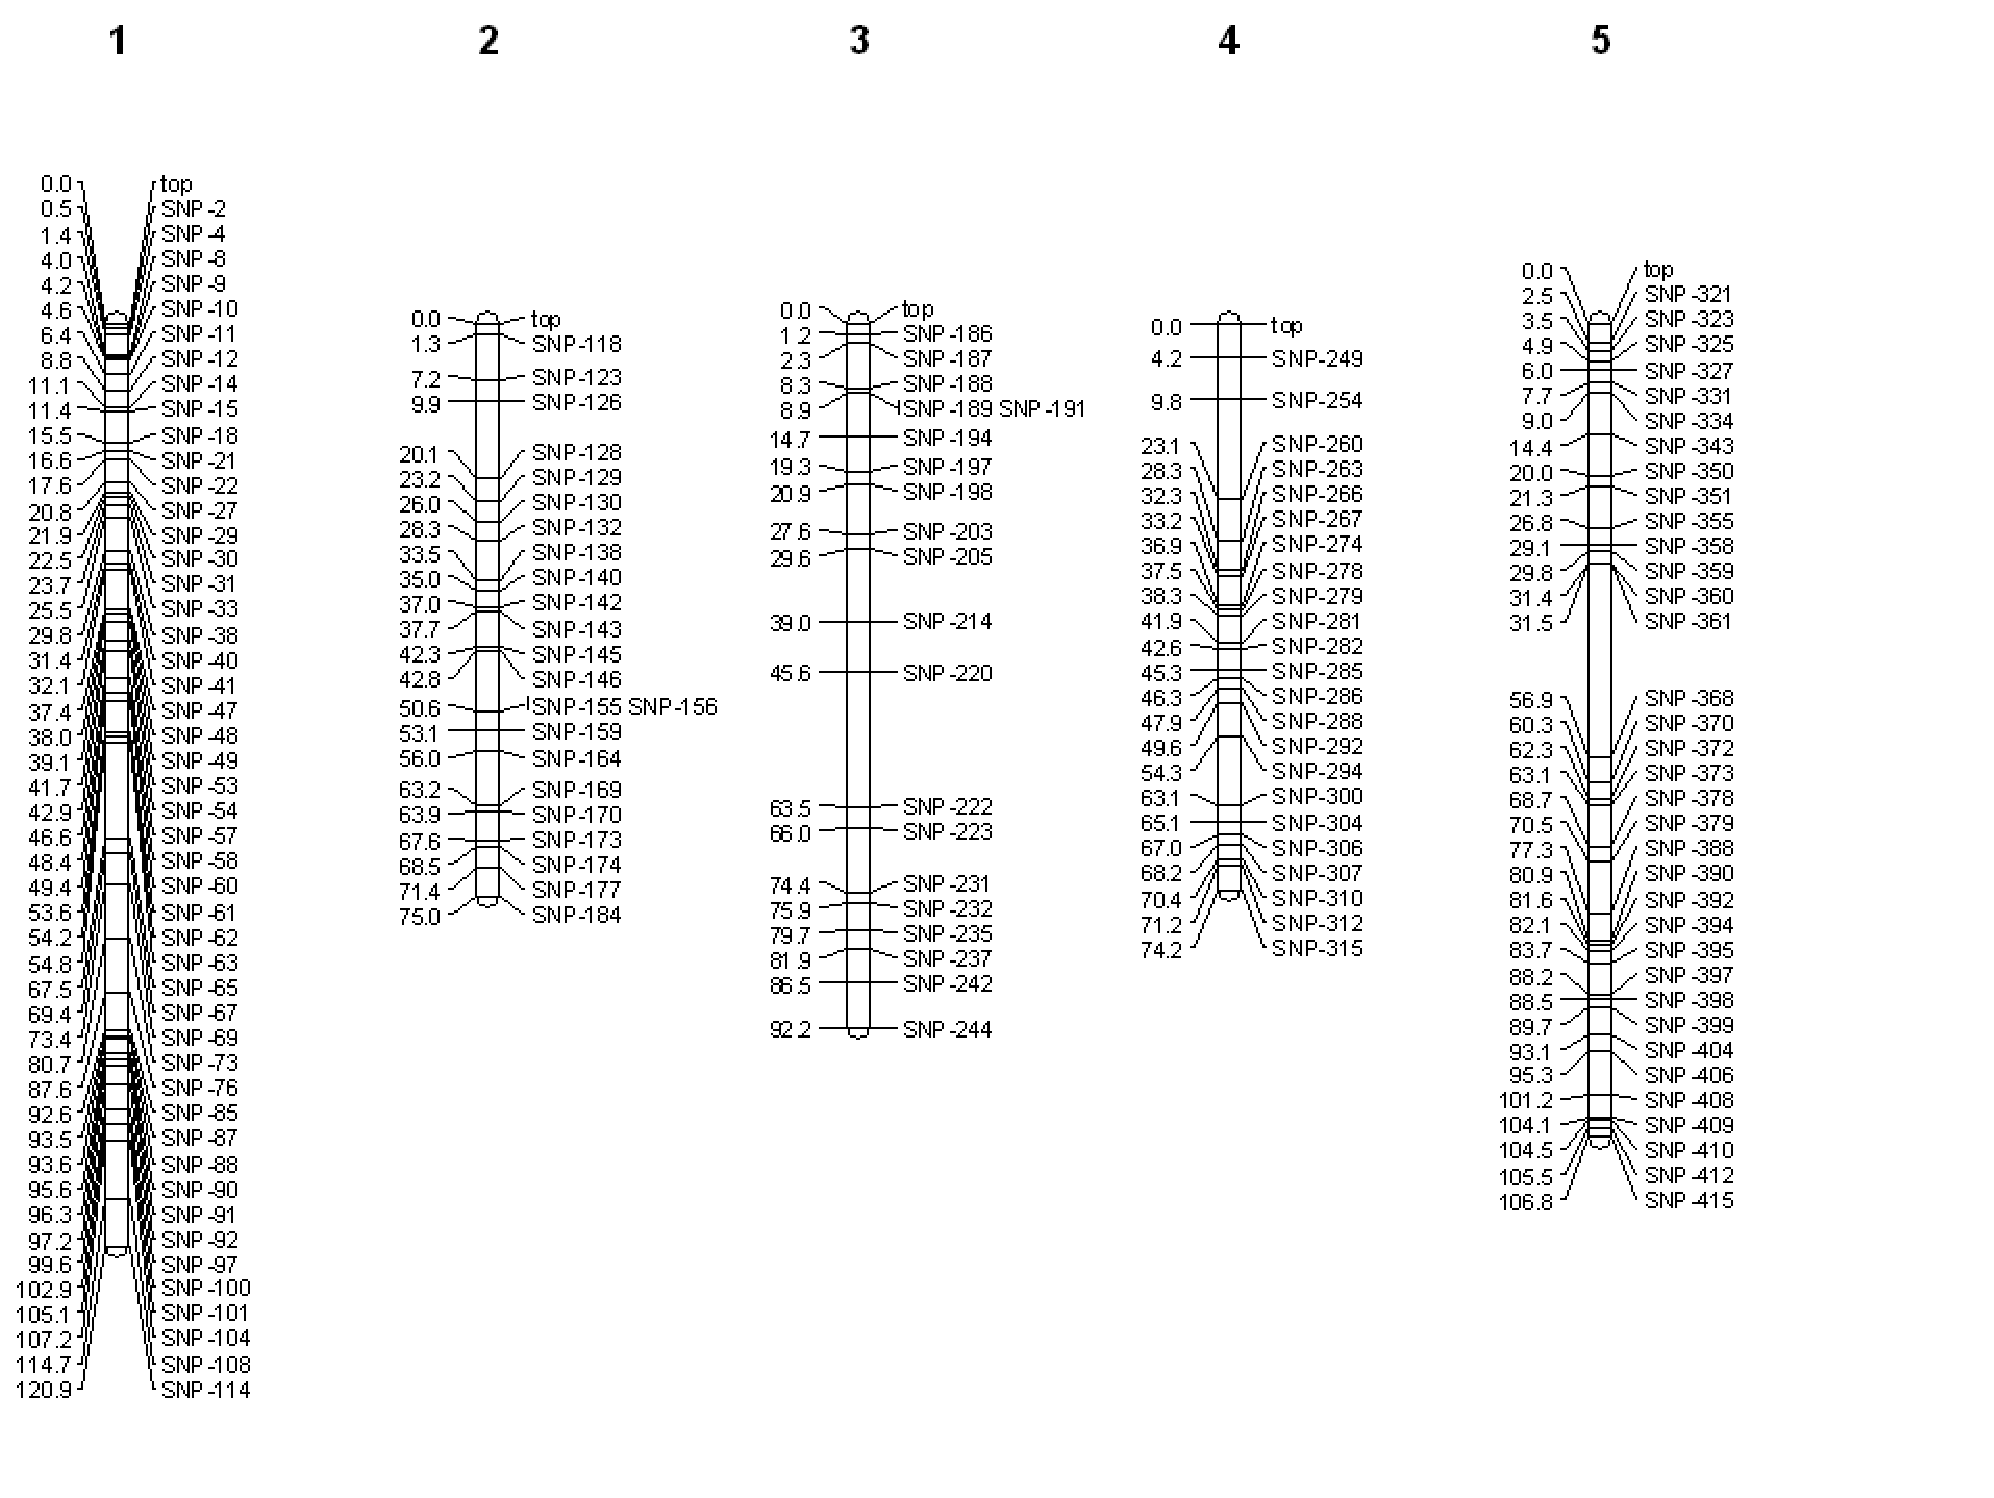
\includegraphics[width=1\textwidth]{figures/snp_locations_on_chr.eps}
\caption{}\label{f1}
\end{figure}


\section{Genotyping Error Rate}
The 96 strains from \cite{Nordborg2005} were genotyped again, which offered an opportunity to have a rough estimate of genotyping error rate by comparing the data from two different experiments. Figure~ is an overview of all the differences.

The optimistic error rate (not counting the NAs) is 121/(12408+121) = 0.96\%. Taking the NAs into account, the error rate would be (121+893+804)/( 12408.0+121+893+804) = 12.78\%.


\section{Bogus Heterozygous Calls(column-wise)}
Figure~\ref{f2} shows the distribution of heterozygous calls in a Strain by SNP matrix. Apparently, there're columns with a number of unreasonable heterozygous calls.

\begin{figure}
\includegraphics[width=1\textwidth]{figures/justin_data_heterozygous.eps}
\caption{}\label{f2}
\end{figure}

A simple statistical model is used to quantitively tell how unreasonable each column is.

\subsection{model for snp locus}
\begin{equation}
P({SNP}_j|Strain\quad heterozygous\quad info) = \prod_{i=1}^{N} p_i^{a_i^j} (1-p_i)^{1-a_i^j}
\end{equation}

$p_i$ is probability that one strain has heterozygous call.

$a_i^j$ is indicator whether ${SNP}_j$ is homozygous($=1$) or not($=0$) for ${Strain}_i$.

Figure~\ref{f3} is the histogram of the probability for each SNP locus after taking logarithm.

\begin{figure}
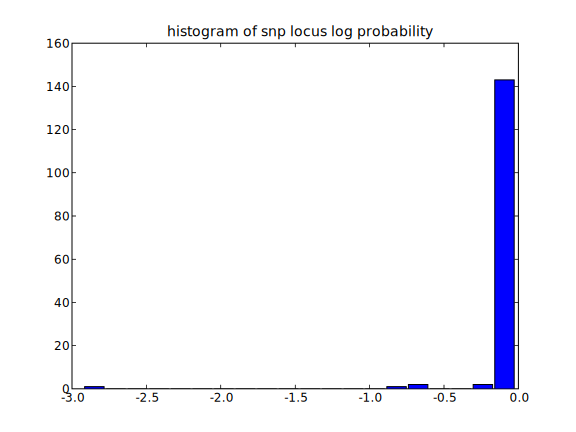
\includegraphics[width=1\textwidth]{figures/justin_data_y_SNP_locus_log_prob.eps}
\caption{}\label{f3}
\end{figure}

4 SNP loci with log probability $\leq -0.5$ were removed. These four loci show long stretch of heterozygous calls among lots of strains in Figure~\ref{f2}.

\section{NA Filtering}
Figure ~\ref{f10} is the Strain by SNP matrix after being sorted. A bunch of NA-rich strains are shown on top of the figure.

\begin{figure}
\includegraphics[width=1\textwidth]{figures/justin_data_y_b.sorted.eps}
\caption{0 is NA. 1-4 is ACGT. 5-10 is heterozygous call}\label{f10}
\end{figure}


Figure~\ref{f4} is a histogram of NA percentage in all SNPs. 3 SNPs with $\geq 40\%$ NAs were removed. Figure~\ref{f5} is a histogram of NA percentage in all strains. 254 strains with $\geq 40\%$ NAs were removed.

\begin{figure}
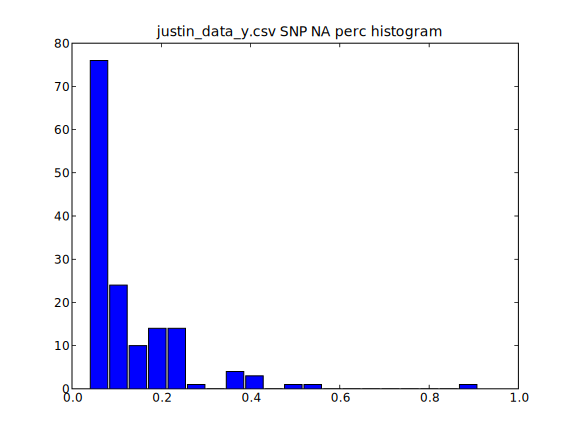
\includegraphics[width=1\textwidth]{figures/justin_data_y_SNP_NA_perc.eps}
\caption{}\label{f4}
\end{figure}

\begin{figure}
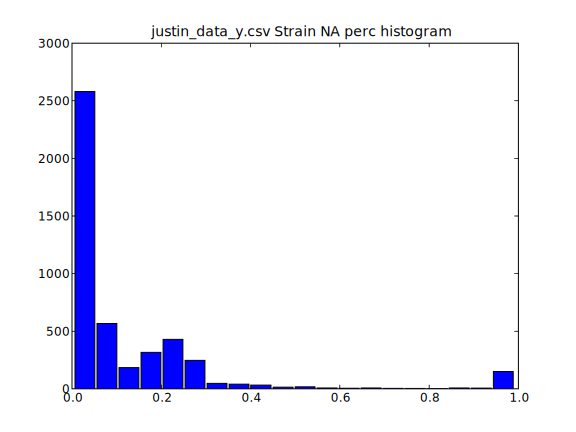
\includegraphics[width=1\textwidth]{figures/justin_data_y_strain_NA_perc.eps}
\caption{}\label{f5}
\end{figure}

\section{Remove Identity Strains}
Due to the highly inbreeding nature of Arabidopsis, there're lots of identity strains in the samples collected from nature. In Figure~\ref{f10}, blocks of identity strains are very obvious. In the detection of identity strains, NA is regarded to be identical to any genotyping call. Because different strains have NAs in different SNP loci, the identity relation is not transitive. For example, A is identical to B and B is identical to C but A might not be identical to C. A graph is constructed with strains as nodes and two nodes are connected if these two strains are deemed as identical. An example graph is shown in Figure ~(?). A greedy algorithm is used to remove nodes with highest degree until no edges left.

In the end, 2575 strains were removed.

\section{Detecting Recombinant Inbred Line(RIL)}
Figure~\ref{f6} is a diagram showing the production of recombinant imbred lines by selfing.

use Dynamic programming to identify RILs with minimum number of recombinations. Regardless of how many selfing generations, the algorithm tells you whether one strain results from the outcrossing of two strains.

This step gives out results flooded with false trios. The 1st kind of false trio is that one parent is very close to the child, the other is a little farther (but still with substantial similarity) and just help to save some few incompatibilites. The 2nd kind is that one parent and child are close. The other parent is kind of irrelevant and saves the incompatibilites by being 'NA'.

\section{Estimate the number of selfing generations since the last outcrossing event}
Figure~\ref{f6} is a diagram showing the production of recombinant imbred lines by selfing. F1 would be 0 selfing generation away from the last outcrossing event as it's the direct result of outcrossing. F2 is 1 selfing generation away from the last outcrossing event.

\begin{figure}
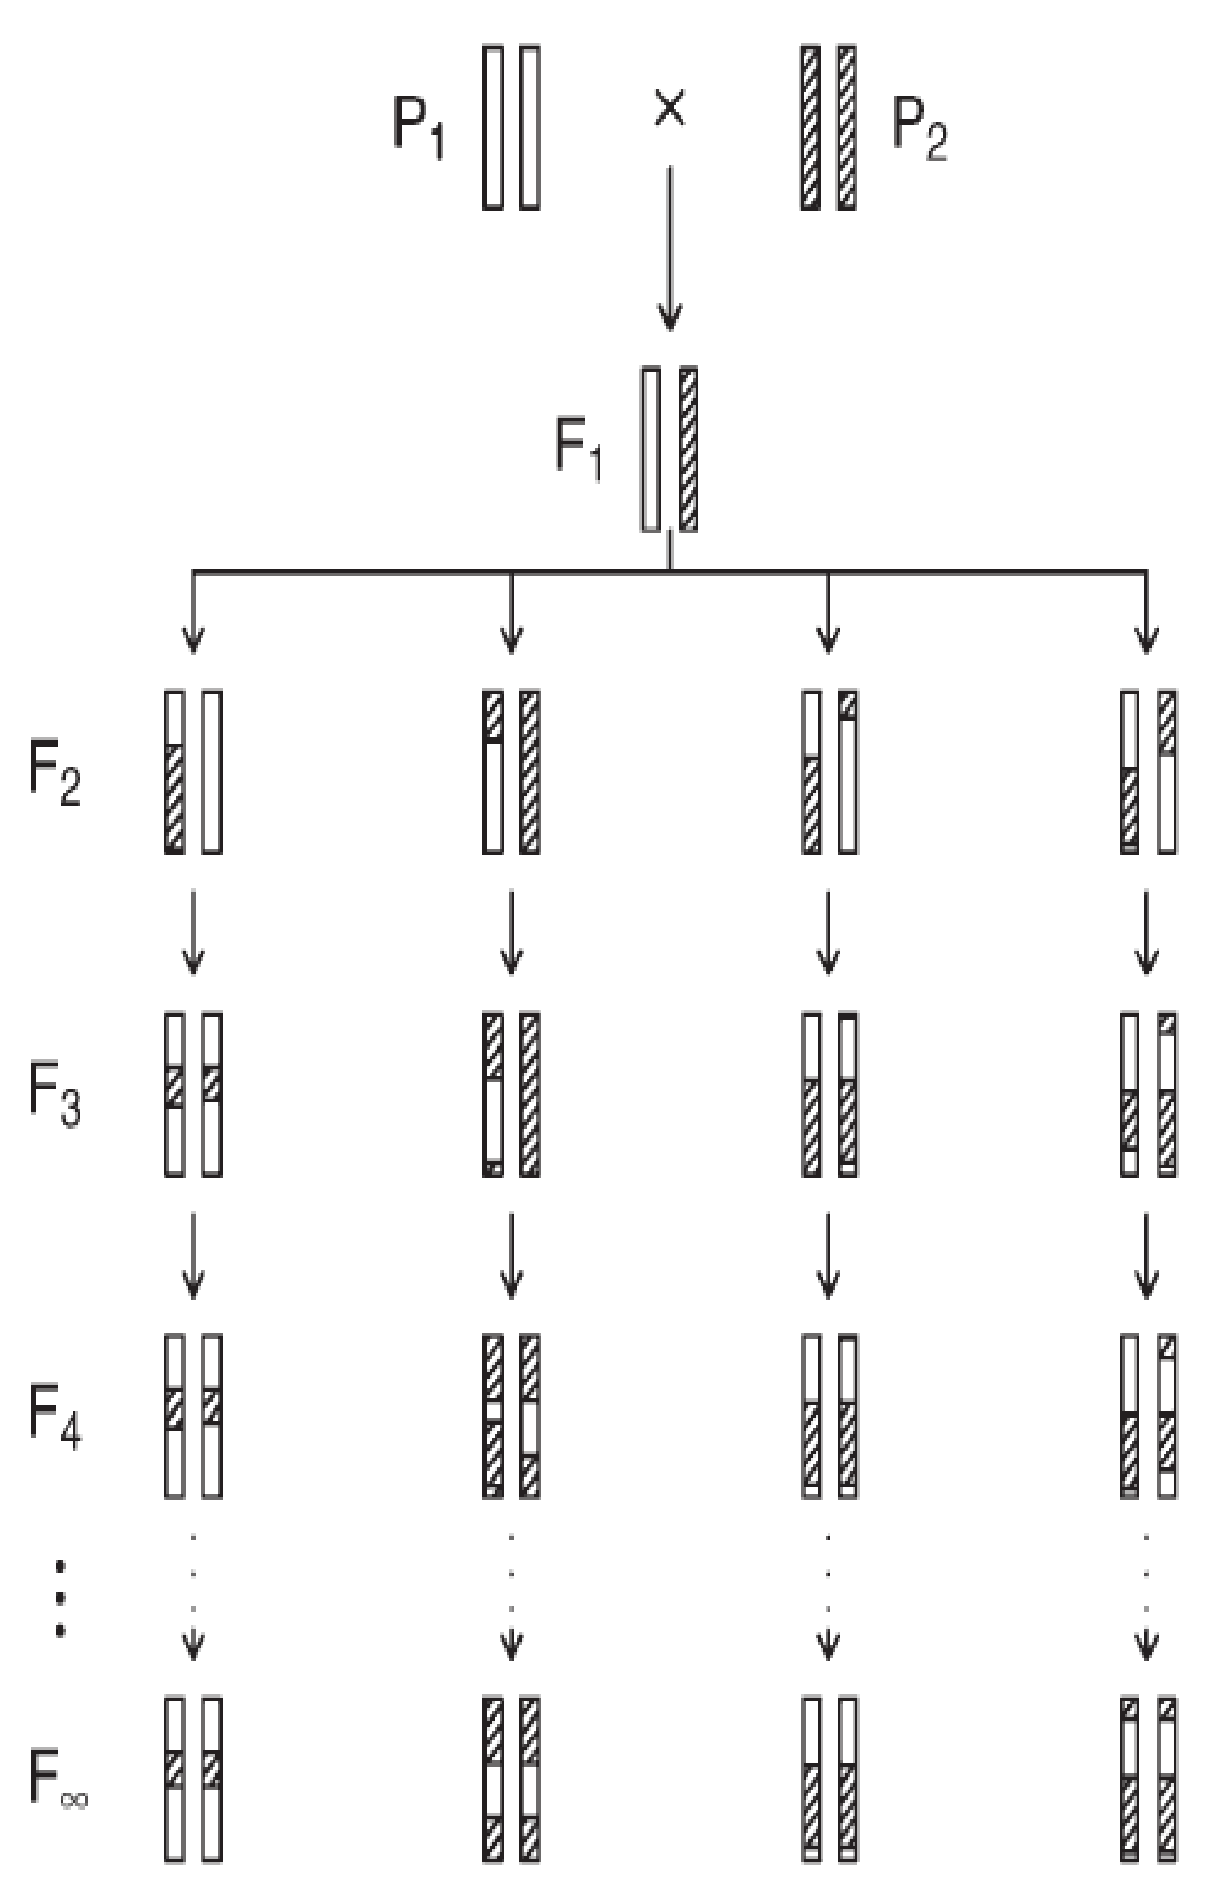
\includegraphics[width=1\textwidth]{figures/selfing_diagram.eps}
\caption{from \cite{Broman2005}}\label{f6}
\end{figure}

The following model is from \cite{Enjalbert2000}.

\subsection{model to estimate the number of selfing generations since the last outcrossing event}
\begin{equation}
D_i = 1 - \sum_{j=1}^k p_{ij}^2
\end{equation}


$p_{ij}$ is probability of allele j of SNP i. k is the number of alleles.

$D_i$ is probability of SNP i being heterozygous.


\begin{equation}
likelihood(S_n) = \prod_{i=1}^L {(\frac{D_i}{2^n})}^{a_i} {(1-\frac{D_i}{2^n})}^{1-a_i}
\end{equation}

$S_n$ is the strain which is n selfing generations away from the last outcrossing event.

$L$ is the number of loci.

$a_i$ is indicator whether SNP i is heterozygous($=1$) or not($=0$).

$\hat{n}$ is the MLE.

This model assumes the independence among the SNP loci, which is not true in general due to LD. According the recent Kim et al.(2007) paper (in preparation), LD decays within 10kb on average. In our data, the spacing between neighboring SNP loci is generally huge (see Figure~\ref{f7}). If sorted, the list of gaps between loci looks like 1713, 4520, 13250, 49053, ..., 4482219, 6334701. So only the first two gaps are within 10kb frame. So statistical independence could be well assumed.

\begin{figure}
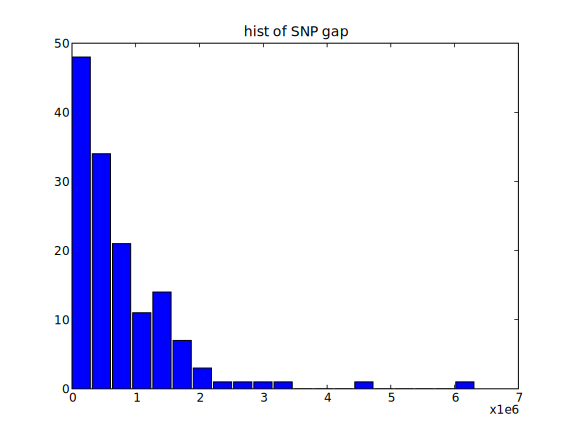
\includegraphics[width=1\textwidth]{figures/snp_locus_gap_hist.eps}
\caption{}\label{f7}
\end{figure}

Figure~\ref{f8} is the result. The spike in 6 is probably spurious estimates.

\begin{figure}
\includegraphics[width=1\textwidth]{figures/justin_data_y_b_filtered.estimate.selfing.generation.hist.eps}
\caption{}\label{f8}
\end{figure}

Figure~\ref{f9} is an example showing one strain with 0 selfing generations from the last outcrossing event.

\begin{figure}
\includegraphics[width=1\textwidth]{figures/trio1.eps}
\caption{}\label{f9}
\end{figure}

\section{Estimate outcrossing rate}
This part is still pending due to the unresolved issue regarding the geographic information of all strains.

\bibliography{outcrossing}
\bibliographystyle{plain}

\end{document}
